\documentclass{../source/zju}

\title{\zihao{4} \bf{快速傅里叶变换的MATLAB实现}}
\author{\zihao{5} }
\date{}

\major{信息工程}
 \name{箫宇 }
\stuid{ }
\college{信息与电子工程学院}
\date{\today}
\instructor{胡浩基}

\begin{document}
\makecover
\maketitle
\begin{abstract}
    \noindent
    {\bf 摘要:}本次大作业采用了非递归的方法实现了基2的快速傅里叶变换算法,并且利用插值的方法实现了长度非$2^n$的序列的傅里叶变换。在数据规模小于$2^{17}$次方时表现良好。本方法一个比较巧妙的点在于利用了一种特别的方法实现了二进制倒序。\\
    {\bf 关键词:}fft
\end{abstract}

\section{问题的提出}
因为LTI系统对复指数信号响应具有一种特别简单的形式,因此将用复指数信号$e^{st}$或者$z^n$作为一类基本信号来表示一般任意信号。然后根据LTI系统的叠加性质,LTI系统对任意一个由这些基本信号的线性组合而成的输入信号的响应就是系统对这些基本信号单个响应的线性组合,这就提供了另一种非常方便的LTI系统分析方法:变换域分析法。

而提及变换频域分析,就不得不提到傅里叶变换了。基于傅里叶变换的频域分析法为信号与系统的分析、设计和理解提供了一种非常有效的基本方法,这使得我们能够从频域的角度获得对信号和LTI系统的性质的更加深入的理解,也使得信号与LTI系统得到了更为广泛的应用。

而随着微电子技术以及数字计算机的出现与发展,使得离散时间信号与系统的具体应用领域得到了很大拓展与发展。20世纪60年代初期,库利和图基提出的快速傅里叶变换算法,使得傅里叶变换的运算量减少了几个数量级,极大地推动了数字信号处理这一学科的发展。直到现在,FFT算法依旧是数字信号处理的经典方法。而本次设计作业,通过自己学习并编写FFT算法,能够极大程度地加深对傅里叶变换的理解和应用,了解计算机进行离散傅里叶变换的过程。

\section{原理及算法}
在查阅了相关资料之后,发现FFT大致分为两类:固定基以及混合基实现。MATLAB中fft便是采用了混合基的方法实现的快速傅里叶变换,这种方法有点在于可以处理非$2^n$个点的傅里叶变换,计算速度较快。但是由于时间的紧迫以及能力的限制,混合基算法我仅了解了相关知识,在实现FFT算法时仍旧选择了基2的算法实现。此种方法的方便之处在于算法实现较为简单,编程实现难度较低,虽然运算速度比不上MATLAB中的fft,但是在编写此种算法的过程中也能够让人体会到FFT的巧妙之处。
\subsection{程序实现方式}
胡老师给的推荐代码中采用的是递归的方式进行实现,但我认为递归的方式虽然编程方式简单,但由于递归算法本身的限制,有着一些不好之处。递归需要调用系统的堆栈,消耗的存储空间会比非递归的方式大很多,而且在递归层数太深,也多了系统崩溃的可能性。相对于递归算法,非递归的方式虽然稍微复杂一点且没有递归的方式容易让人理解,但它的执行时间仅与循环的次数有关,没有太多的额外开销,同时也节约了创建新的空间的时间,效率更高。

在利用蝶形图作为编程工具之后,代码的编写难度已经得到了很大程度的减小,所以在经过一系列权衡之后,我决定采用非递归的方式进行实现,最后结果也证明了这能够极大地减少程序的运行时间
\subsection{编码倒序的实现}
因为程序选用了非递归的方法实现,编码倒叙的实现就不能像递归一样很自然地奇偶分离了,在此处,利用倒叙后二进制代码的特征,采用了一种非常巧妙的方法将其实现。因为MATLAB中移位操作符被用作了别的用途且数组下标从1开始,介绍算法时采用C语言代码。
\begin{lstlisting}[
    language = c
]
    static int rev[X];//X为序列长度
    for(int i=0;i<X;i++)
        rev[i]= (rev[i>>1]>>1)|((i&1)<<(K-1)) ;//K为二进制编码的位数
\end{lstlisting}
首先我们初始化一个长为X的全0数组,以3位二进制数为例,观察序列我们可以发现x的倒叙的低2位刚好为x>>1倒叙的高2位,所以我们可以通过将x>>1的二进制编码右移一位得到x处的低2位;至于x的最高位,我们将x与1取与就可得到,将其左移2位于上一步的结果取或就得到了x的倒叙序列.通过循环,我们在计算x处值时,前x个数的倒叙已经计算得出,所以此算法能够实现。

例子:求3的倒叙

$\because  i = 3 ;3>>1 = 1$

$\therefore rev[i>>1] = rev[1] >> 1 = 010 ,(3\&1)<<2 = 100$

$\therefore rev[3] = 010 | 100 = 110$

结果正确。
\newpage
\begin{table}[htp]
    \centering
    \begin{tabular}{|c|c|c|}
    \hline
    序号 & 二进制 & 倒序后二进制 \\ \hline
    0  & 000 & 000    \\ \hline
    1  & 001 & 100    \\ \hline
    2  & 010 & 010    \\ \hline
    3  & 011 & 110    \\ \hline
    4  & 100 & 001    \\ \hline
    5  & 101 & 101    \\ \hline
    6  & 110 & 011    \\ \hline
    7  & 111 & 111    \\ \hline
    \end{tabular}
    \end{table}

    在利用MATLAB实现时,由于MATLAB寻址从1开始,并且移位操作不够方便,在其中一部分代码我采用 了除2,向下取整然后强制类型转换的方式实现,代码如下:
    \begin{lstlisting}[
        language = matlab
    ]
    rev = zeros(length_after_add_zero);
    for i = 0:1:length_after_add_zero-1
        rev(i+1) = bitor(int32(floor( (rev( floor(i/2)  + 1 ))/2 ) ) , bitshift(int32(bitand(int32(i),1)), bit_counter-1)) + 1;
    end
    \end{lstlisting}

    \subsection{蝶形运算设计}
    \begin{figure}[thp]
        \centering
        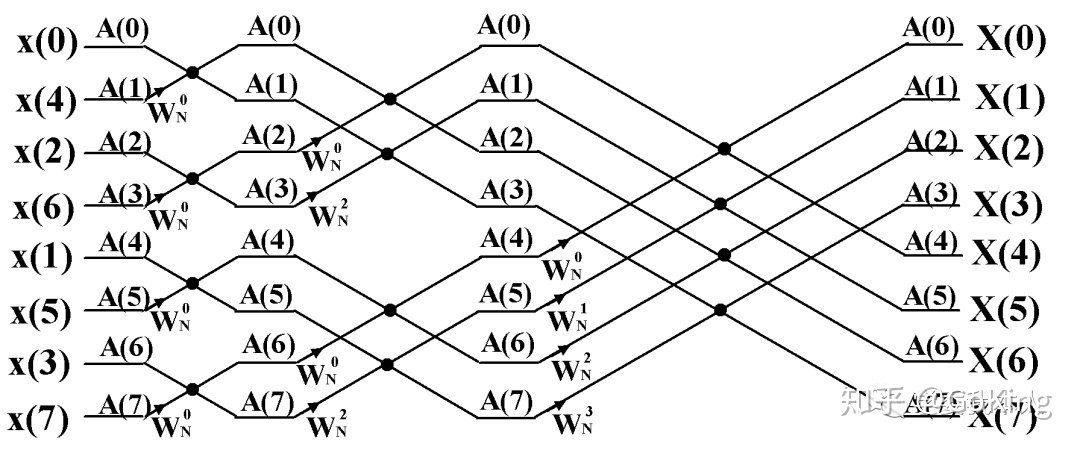
\includegraphics[width = 0.9\textwidth]{figure/蝶形图.jpg}
        \caption{蝶形图}
    \end{figure}
    定义旋转因子:$W_N^P = e^{-j\frac{2\pi}{N}P}$

    按照蝶形图从左向右编程,L为蝶形运算的层数,B为每个蝶形运算输入的两个数据的间隔,P则是旋转因子的P值,下文中的代码便能实现bit_counter层的蝶形图。
    \begin{lstlisting}[
        language = matlab
    ]
    for L = 1:1:bit_counter
        B =int32(pow2(L-1));
        for m = 0:1:B-1
            k = int32(pow2(bit_counter - L));
            P = m*k;
            for i = 0:1:k-1
                r = m + 2*B*i;
                temp = x(r+1);
                x(r+1) = x(r+1) + x(r+B+1) * exp(-1j*double(2*pi*double(P)/double(length_add)));
                x(r+B+1) = temp - x(r+B+1) * exp(-1j*double(2*pi*double(P)/double(length_add)));               
            end
        end
    end
    \end{lstlisting}


    \subsection{实现非$2^n$个点的FFT}
    因为采用了基二的傅里叶算法,这就导致了无法实现非$2^n$个点的傅里叶变换,在处理这一点时,我采取了补零的方法实现。

    课上我们学到,补零之后频域图的包络并不会发生改变,所以我们可以在补零之后利用插值的方法求出非$2^n$个点的傅里叶变换,插值时采用了最为简单的一次插值。在点的数目较少时,这会带来较大的误差,为了尽可能减少这一误差,我至少将序列补零至了$2^{10}$个点,这虽然带来了一定的时间消耗,但就算是只有3个点的傅里叶变换,也能保证小数点后4为和MATLAB提供的fft函数计算出的值完全相同,我个人认为此处带来的时间消耗是值得的。具体代码如下:

    \begin{lstlisting}[
        language = matlab
    ]
    if(length_after_add_zero ~= length_x)
    for m = 1:1:length_x
        number = floor(double((m-1)*length_after_add_zero)/double(length_x));
        after = double(number+1)/double(length_after_add_zero);
        before = double(number)/double(length_after_add_zero);
        this = double(m-1)/double(length_x);
        Y(m) = (after-this)*x(number+1)*double(length_after_add_zero) + (this - before)*x(number+2)*double(length_after_add_zero);
    end
    end
    \end{lstlisting}

\section{验证}
    \subsection{代码}
    \begin{lstlisting}[
        language = matlab
    ]
    clc
    clear
    %%
    N=128,A0=255;PI=3.1415926;
    i=1:N;
    x=A0 * (sin(2*PI*i/25)+sin(2*PI* i * 0.4 ));
    tic;
    y=fft(x,N);%进行傅里叶变换求得幅度谱
    toc;
    z=abs(y);%对求得的幅度谱加绝对值   
    figure(1);
    subplot(2,2,1);plot(i,x);title('时域图');
    subplot(2,2,2);plot(i,z);title('MATLAB自带fft测试结果')
    tic;
    var2 = fftNew(x);
    toc;
    subplot(2,2,3);plot(i,x);title('时域图');
    subplot(2,2,4);plot(i,abs(var2));title('自己所写fftNew测试结果');
    %%
    N=234,A0=255;PI=3.1415926;
    i=1:N;
    x=A0 * (sin(2*PI*i/25)+sin(2*PI* i * 0.4 ));
    tic;
    y=fft(x,N);%进行傅里叶变换求得幅度谱
    toc;
    z=abs(y);%对求得的幅度谱加绝对值   
    figure(2);
    subplot(2,2,1);plot(i,x);title('时域图');
    subplot(2,2,2);plot(i,z);title('MATLAB自带fft测试结果')
    tic;
    var2 = fftNew(x);
    toc;
    subplot(2,2,3);plot(i,x);title('时域图');
    subplot(2,2,4);plot(i,abs(var2));title('自己所写fftNew测试结果');
    \end{lstlisting}
    
    \subsection{$N=2^n$时正确性验证}
    由下图可以看出,在$N=2^n$时,fftNew计算出的结果和fft函数结果一样,结果正确。
    \begin{figure}[thp]
        \centering
        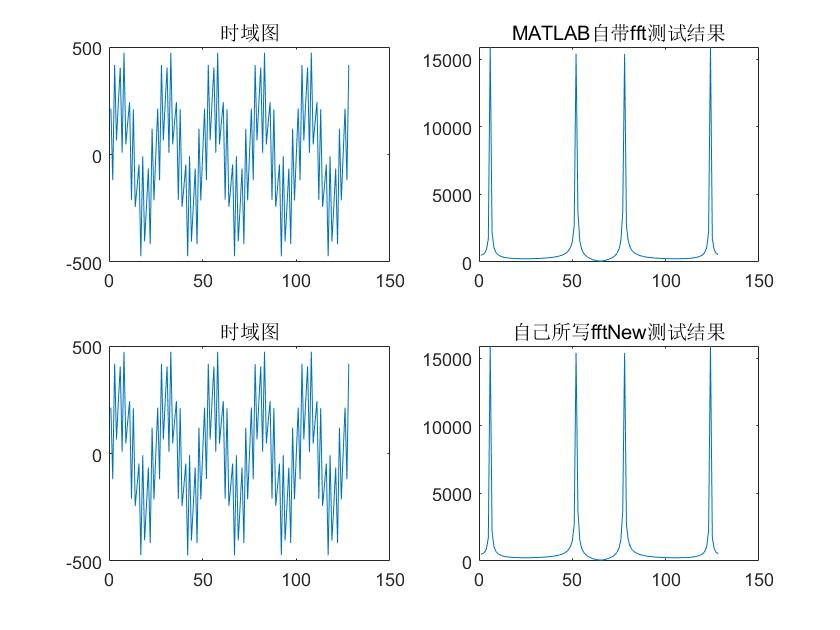
\includegraphics[width = 0.8\textwidth]{figure/正确性验证.jpg}
        \caption{$N=2^n$}
    \end{figure}

    \subsection{$N!=2^N$时正确性验证}
    由下图可以看出,当$N!=2^N$时结果正确
    \begin{figure}[thp]
        \centering
        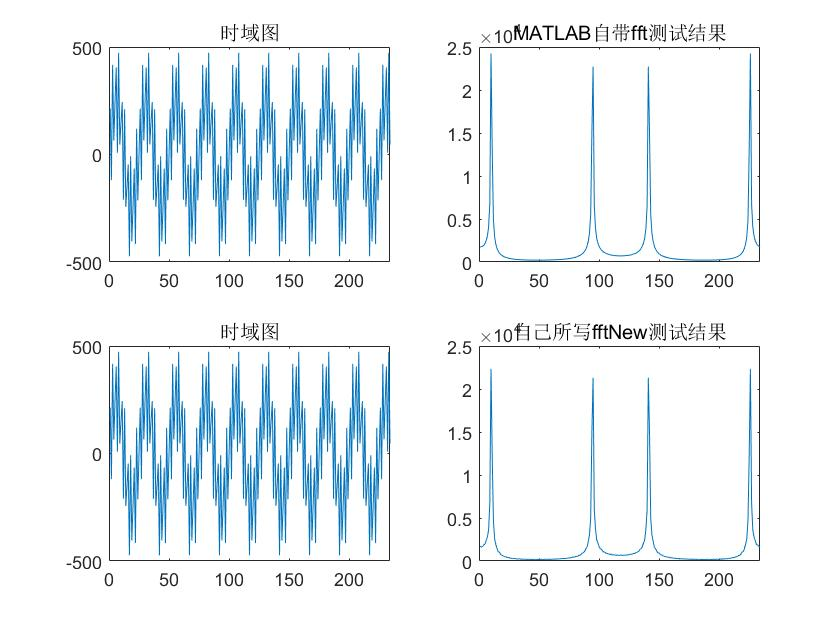
\includegraphics[width = 0.8\textwidth]{figure/N=234.jpg}
        \caption{$N!=2^n$}
    \end{figure}

    \subsection{运行时间}
    第一个时间为系统fft耗时,第二个时间为fftNew耗时,运行时间较为理想。
    \begin{figure}[thp]
        \centering
        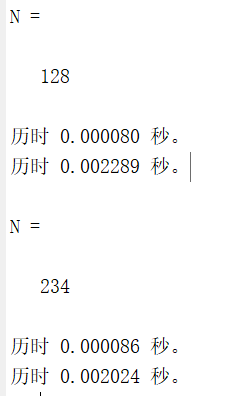
\includegraphics[scale = 0.3]{figure/时间.png}
        \caption{$运行时间$}
    \end{figure}

\section{结论}
通过上述的验证可以发现,自己编写的fft函数正确性能够经受住考验,不过相较于MATLAB中的fft,在运行速度上就是硬伤了。而且,除了运行速度,当数据规模达到$2^17$次方时就没法计算了。
\end{document}